	
\chapter{Sprint 1}
\label{Sprint1}
\lhead{Chapter 7. \emph{Sprint 1}}

\section{Duration}
The duration of this sprint was the following:
\begin{itemize}
\item Start: September, 9th
\item Milestone M1 (first product prototype): September, 20th
\item End: September, 22nd
\end{itemize}

\section{Planning}

After the initial sprint we had come to a general understading of the problem and a \'big picture\' of what our solution would consist of. 
However, we were unsure about what technologies to use for the implementation. 
To address this matter, we tasked one team member with additional studies and set a deadline of four days to choose what technologies to use.
This was done to leave enough time, in view of the impending deadline, to work on an initial design and implementation of a first product prototype which would have included:
\begin{enumerate}
\item the back-end, implementing the logic of the API
\item a database, implementing persistency
\item the front-end, implementing the graphical user interface
\item an Android application to measure heart rate.
\end{enumerate}

Last sprint we had identified two measurements to be used in prototype applications.
We chose to begin implementing an application to measure heart rate because we had found an open-source project which covered most of its required functionality, allowing us to concentrate on implementing interoperability with our back-end (NIPEN).

At the beginning of this sprint our plans for the product consisted in developing, with the following priority:
\begin{enumerate}[1.]
\item an Android app. To measure heart rate
\item an Android app. Using Withings weighing scale
\item an eventual third application interoperable with HealthVault
\end{enumerate}
other than the integration platform itself and its graphical front-end.

\section{Goal(s)}

The goal of this sprint was the completition of an initial prototype of the product whose functionality had to be demonstrated to the customer.
This corresponded to project milestone M1.
The purpose of such demonstration was to act as a proof-of-concept and give the customer a chance to express some feedback upon which we hoped to start a discussion on possible improvements and new features.

Additional goals were the completion of project's planning and documents such as:
\begin{enumerate}[a)]
\item system requirements (both functional and non-functional)
\item report's table of contents
\item concrete work plan
\item risk analysis
\item test plan
\end{enumerate}


\section{Results and feedback}

Around the end of this sprint, on September 20th, we demonstrated a prototype of the product to
the client which included: the front-end, the back-end and an Android application to measure heart rate using the phone's camera.

The backend supported web API calls for storing and retrieving heart rate measurements.
Both the Android application and the front-end used these API calls for sending and retrieving such measurements respectively.
The measurements were ultimately shown to the user on a webpage (the front-end) using a bar chart.
We opted for MySQL as a database to implement persistency on the back-end due to the familiarity we had with it. 
We deployed it on the server machine and added a table so that we could test the web API.
The customer was pleased with the results, stating that they were above his expectations.

We discussed about what he would like to see implemented next in the product between interoperability with Withings or HealthVault and we agreed to prioritise the latter.
The reason behind this decision was the fact that it would have enabled the product to use third-party devices supported by HealthVault to gather health data.
Since the number of devices supported by HealthVault is substantial \footnote{HealthVault supports more than 200 devices in the U.S.}, this was deemed a desiderable feature for the product.

The customer asked if the amounts of resources we had at disposal to actually implement such interoperability was sufficient and inquired about the general viability of such approach.
We expressed our confidence about its feasibility and that the resources at hand were sufficient.
Nevertheless, we set a deadline (10 days) to assess its praticality in order not to delay the general progress of the product.
Furthermore, we anticipated the customer that next sprint's focus would have been writing documentation in view of the midterm report delivery milestone.

\textbf{Notes}: by the end of the sprint one team member had found a job and moved permanently to Oslo.
He expressed his continued committment to the project and told the other members that he would continue to contribute to the project remotely.

\section{Evaluation}

\begin{figure}
\centering
\includegraphics[scale=0.60]{../Figures/burndownSprint1.png}
\caption{Iteration burndown chart}
\label{figure:burndownsprint1}
\end{figure}

The sprint was successful as we managed to achieve the main goal of the sprint (Milestone M1).
We were pleased by the positive feedback received from the customer and felt motivated to keep up the good work. 
Furthermore, having proactively partecipated in the improvement/proposal of product requirements together with the customer made the whole team look forward to implement these new features and improve the product. 
Although we didn't manage to write anything in the report we still had enough time ahead to make up for it so we consider that a minor issue.
Development times for the Android application were dramatically reduced thanks to the functionality offered by android-heart-rate-monitor (described in section \ref{subsec:hr}).
This iteration's burndown chart (figure \ref{figure:burndownsprint1}) shows that development proceeded quicker than planned but we still had some tasks left (documentation) uncompleted by the end of the sprint.

\begin{figure}[H]
\centering
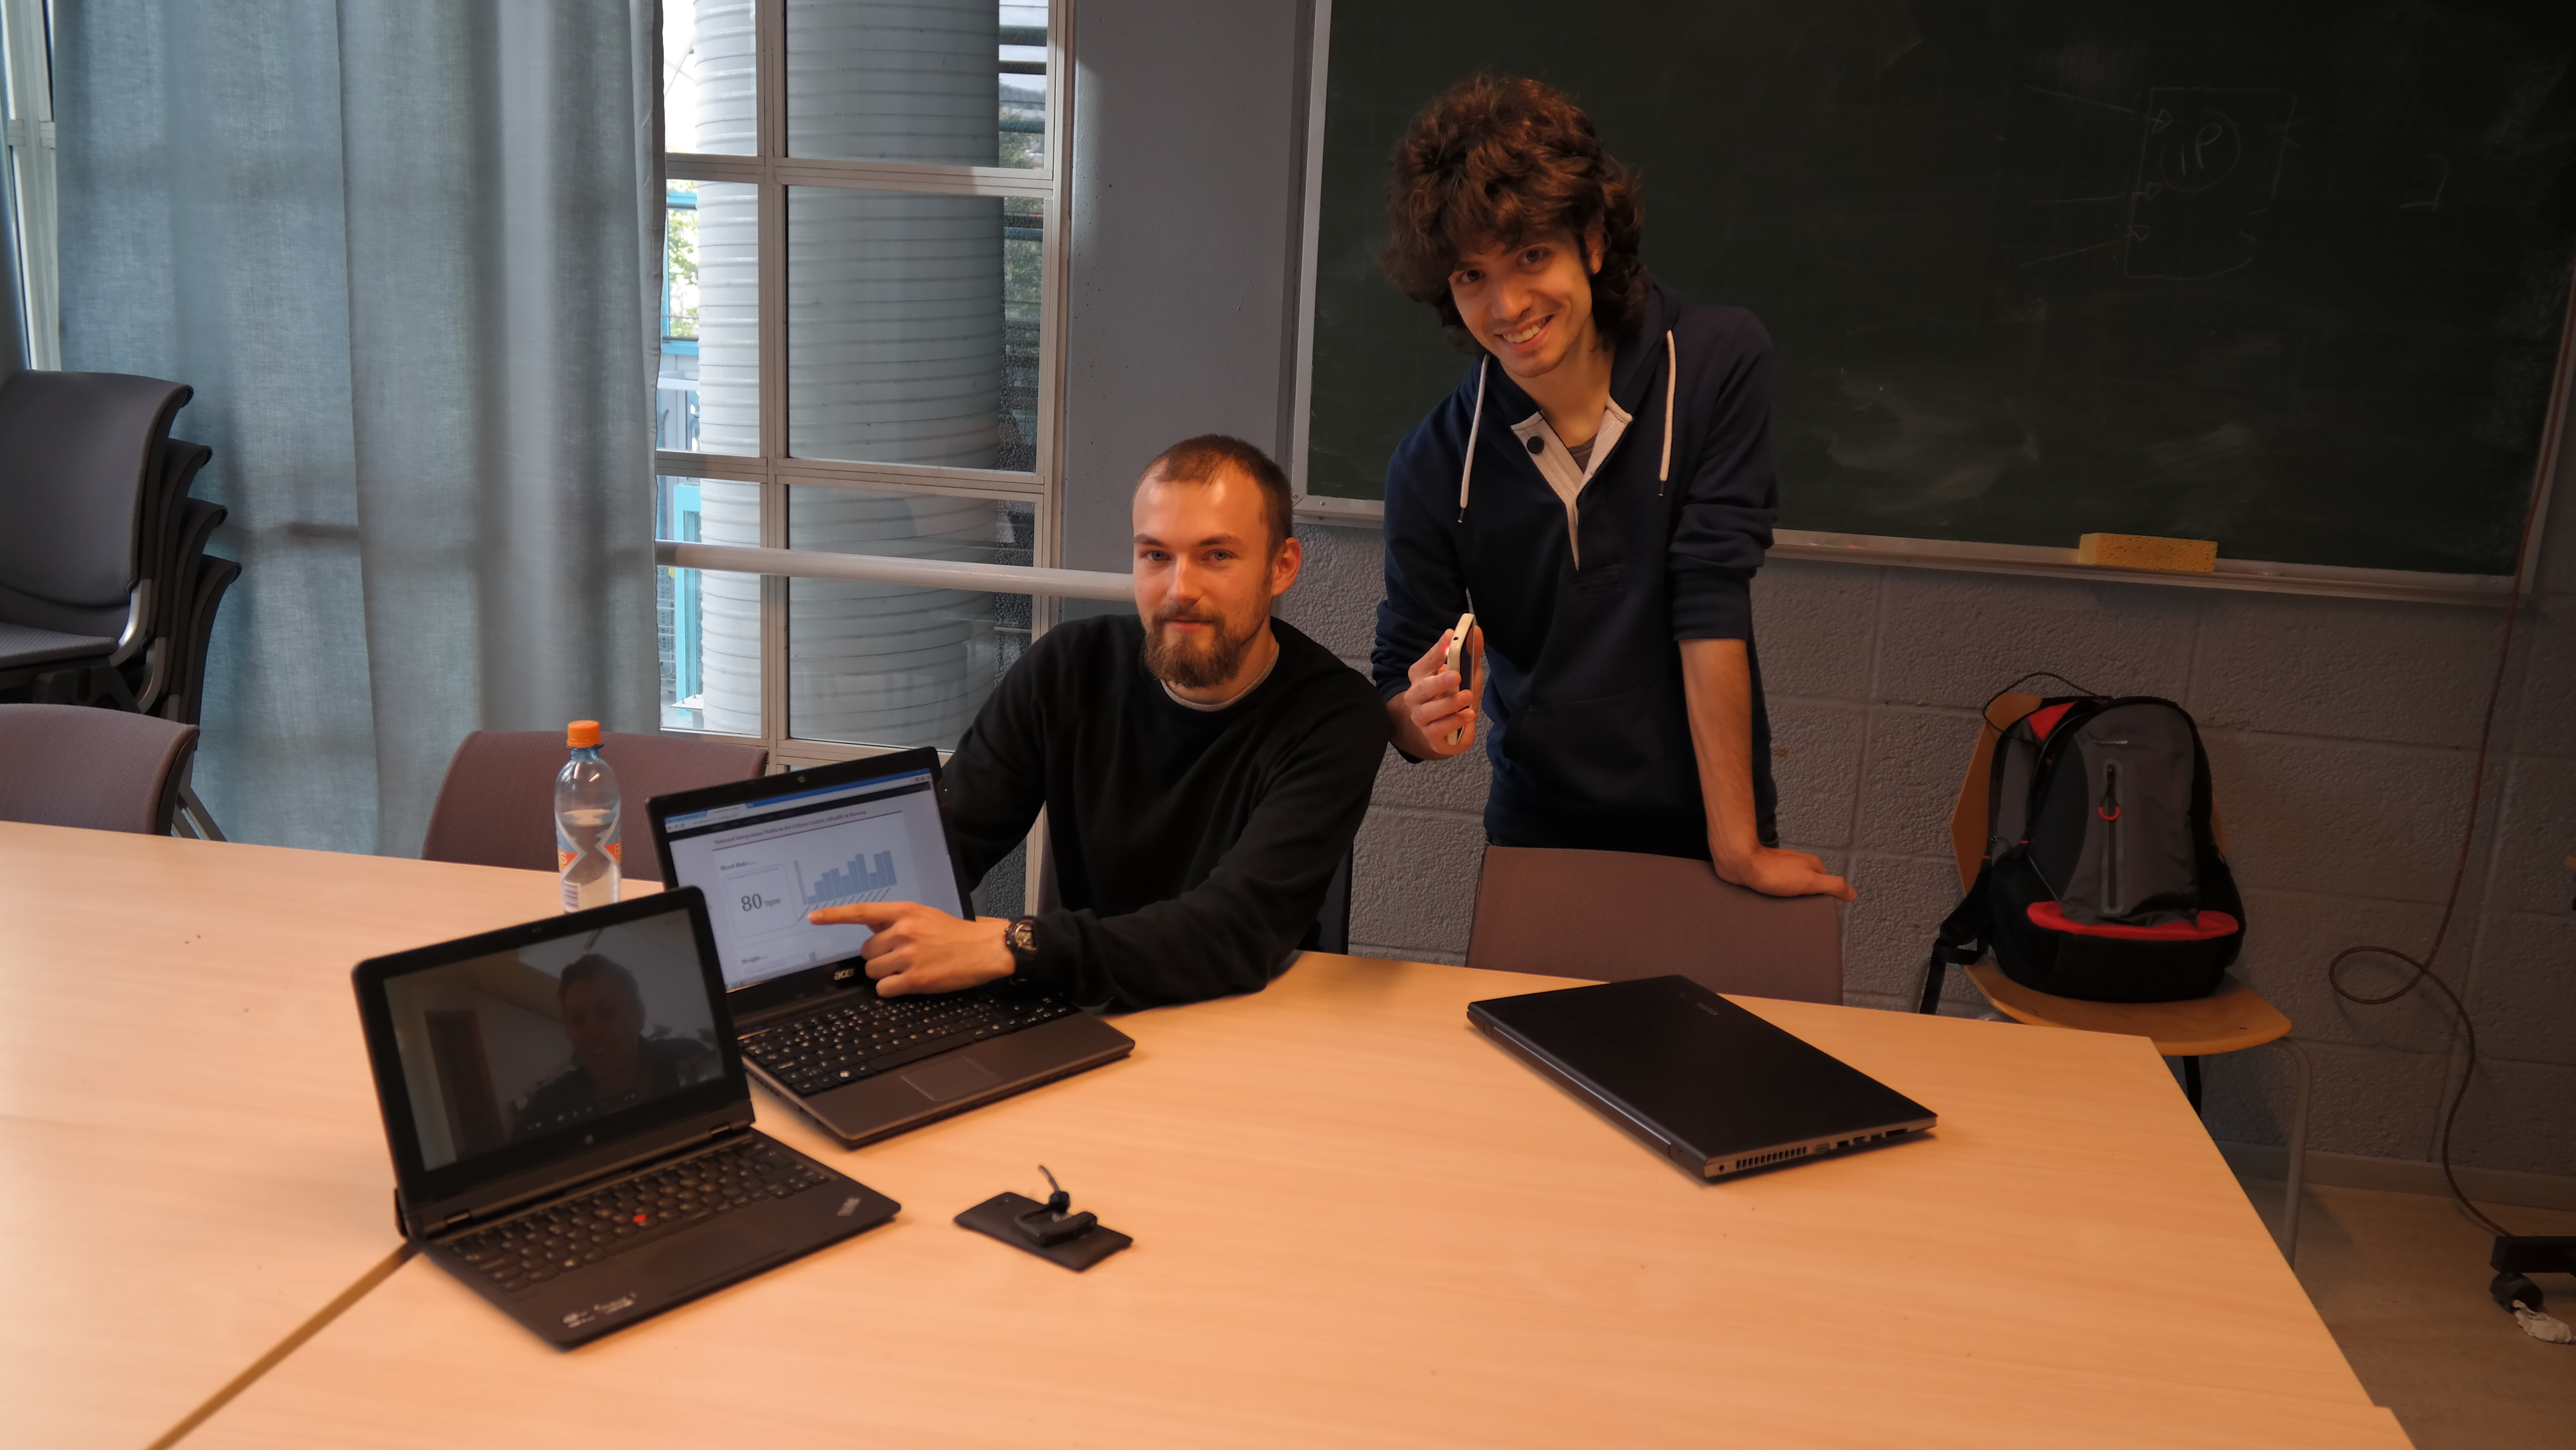
\includegraphics[scale=0.40]{../Figures/demo-m1.jpg}
\caption{Team demonstrating the product}
\label{figure:demonstration-m1}
\end{figure}

Figure \ref{figure:demonstration-m1} shows the team demonstrating the product to the customer (who took the picture).
Emanuele is holding his mobile phone running the heart rate application while Sebastian is pointing at the front-end showing how the data is being acquired. 
Anders is participanting to the conversation through Skype.

\clearpage
\section{Backlog}

See below the sprint backlog.
\begin{enumerate}[1.]
	\item \textbf{M1 First product prototype}:\newline
		a first prototype of the product to be demonstrated to the customer
	\item \textbf{Project management} included:
		\begin{itemize}
			\item \textbf{Sprint startup meeting}:
				included sprint planning and review
			\item \textbf{Weekly meetings}:
				with both the customer and the supervisor
				%The meeting with the customer was held on Skype.
			\item \textbf{Meeting notes}:
				taking notes during meetings, reviewing of the notes
			\item \textbf{Status reports}:
				for both week 37 and 38
			\item \textbf{Risk analysis}:
				updated on a weekly basis
				%The risk analisys was submitted to the supervisor and the customer.
		\end{itemize}
	\item \textbf{Additional pre-studies} on relevant technlogies such as:
	\begin{itemize}
		\item \textbf{HealthVault}: Microsoft's online health platform
		\item \textbf{Apache Camel}: a routing engine for enterprise integration patterns
		\item \textbf{Javascript libraries for charts}: to be used in the frontend
	\end{itemize}
	\item \textbf{System development}: initial design and implementation. This accounted for:
	\begin{itemize}
		\item \textbf{Backend development}:
			coding of Spring controllers for API endpoints
		\item \textbf{Frontend development}:
			set up an web page that performs API calls to fetch heart rate measurements
			and shows them using bar charts
		\item \textbf{Deployment}:
			of both backend and frontend using a servlet container (Tomcat)
	\end{itemize}
	\item \textbf{Heart rate application development}\newline
		basic implementation of the heart rate application. The application should be able to acquire
		the user's heart reate and send perform an API call to store the data on the backend
	\item \textbf{Database development}\newline
		choose a suitable database to use for implementing persistency on the backend.
		Deploy the database and create a table for the heart rate
	\item \textbf{Testing}\newline
		perform unit and integration testing for the heart rate application and the backend
\end{enumerate}